%%%%%%%%%%%%%%%%%%%%%%%%%%%%%%%%%%%%%%%%%
% Beamer Presentation
% LaTeX Template
% Version 1.0 (10/11/12)
%
% This template has been downloaded from:
% http://www.LaTeXTemplates.com
%
% License:
% CC BY-NC-SA 3.0 (http://creativecommons.org/licenses/by-nc-sa/3.0/)
%
%%%%%%%%%%%%%%%%%%%%%%%%%%%%%%%%%%%%%%%%%

%----------------------------------------------------------------------------------------
%	PACKAGES AND THEMES
%----------------------------------------------------------------------------------------

\documentclass{beamer}

\mode<presentation> {
	
	% The Beamer class comes with a number of default slide themes
	% which change the colors and layouts of slides. Below this is a list
	% of all the themes, uncomment each in turn to see what they look like.
	
	%\usetheme{default}
	%\usetheme{AnnArbor}
	%\usetheme{Antibes}
	%\usetheme{Bergen}
	%\usetheme{Berkeley}
	%\usetheme{Berlin}
	%\usetheme{Boadilla}
	%\usetheme{CambridgeUS}
	%\usetheme{Copenhagen}
	%\usetheme{Darmstadt}
	%\usetheme{Dresden}
	%\usetheme{Frankfurt}
	%\usetheme{Goettingen}
	%\usetheme{Hannover}
	%\usetheme{Ilmenau}
	%\usetheme{JuanLesPins}
	%\usetheme{Luebeck}
	\usetheme{Madrid}
	%\usetheme{Malmoe}
	%\usetheme{Marburg}
	%\usetheme{Montpellier}
	%\usetheme{PaloAlto}
	%\usetheme{Pittsburgh}
	%\usetheme{Rochester}
	%\usetheme{Singapore}
	%\usetheme{Szeged}
	%\usetheme{Warsaw}
	
	%\bibliographystyle{abbrvnat}
	\bibliographystyle{plain} % reference type change : [1] , [2] , ... (+ usepackage(natbib))
	% As well as themes, the Beamer class has a number of color themes
	% for any slide theme. Uncomment each of these in turn to see how it
	% changes the colors of your current slide theme.
	
	%\usecolortheme{albatross}
	%\usecolortheme{beaver}
	%\usecolortheme{beetle}
	%\usecolortheme{crane}
	%\usecolortheme{dolphin}
	%\usecolortheme{dove}
	%\usecolortheme{fly}
	%\usecolortheme{lily}
	%\usecolortheme{orchid}
	%\usecolortheme{rose}
	%\usecolortheme{seagull}
	%\usecolortheme{seahorse}
	%\usecolortheme{whale}
	%\usecolortheme{wolverine}
	
	%\setbeamertemplate{footline} % To remove the footer line in all slides uncomment this line
	\setbeamertemplate{footline}[page number] % To replace the footer line in all slides with a simple slide count uncomment this line
	
	\setbeamertemplate{navigation symbols}{} % To remove the navigation symbols from the bottom of all slides uncomment this line
}
\setbeamertemplate{caption}[numbered]{} % figure number attached : figure 1 , 2 ,...
\usepackage{natbib} % reference type change : [1] , [2] , ... 
\usepackage{graphicx} % Allows including images
\graphicspath{{./img/}}
\usepackage{caption}
\usepackage[normalem]{ulem} % cancel line. when you input the ulem.sty in your file package will work on.
\usepackage{subcaption}
\usepackage{booktabs} % Allows the use of \toprule, \midrule and \bottomrule in tables
\usepackage{amsmath}
\usepackage{amssymb}
\usepackage{amsthm}
\usepackage{animate} % after converting gif to png file by means of the imagemagic display program... (install - ocgbase.sty,pdfbase.sty,animate.sty)
%\usepackage {tikz}
\usepackage{tkz-graph}
\usepackage {xcolor}
\definecolor {processblue}{cmyk}{0.96,0,0,0}

%----------------------------------------------------------------------------------------
%	TITLE PAGE
%----------------------------------------------------------------------------------------

\title[Short title]{5. Weight Initialization}

\author{Dong-Gyu, Lee}
\institute[] % Your institution as it will appear on the bottom of every slide, may be shorthand to save space
{
	Dept. of Statistics, KU% Your institution for the title page
	\medskip
}
\date{2020, Mar 10} % Date, can be changed to a custom date

\begin{document}
	
	\begin{frame}
		\titlepage % Print the title page as the first slide
	\end{frame}
	
	\begin{frame}{Contents}
	\frametitle{Contents}
		\tableofcontents 
	\end{frame}
	
	%----------------------------------------------------------------------------------------
	%	PRESENTATION SLIDES
	%----------------------------------------------------------------------------------------
	\section{Today's Goal}
	\begin{frame}{Today's Goal}
		\begin{itemize}
			\item In this time, we will focus on the various initializing methods.
			\item And we will look at the characteristics of each method through a formula and a picture.
		\end{itemize}
	\end{frame}


	\section{Importance of initialization}
	\begin{frame}{Importance of initialization}
		\begin{itemize}
			\item We obtain the appropriate $W$ (often called the parameter matrix) from training a model in MLP, CNN, RNN, etc.
			\item Because of the large number of parameters, we can't set all of them individually.
			\item So many people start thinking about various methods how to simply initialize the parameters.
		\end{itemize}
	\end{frame}	
		
		
	\begin{frame}{Importance of initialization}
		\begin{itemize}
			\item If all of the initial values are 0, there is no learning of the parameters.
			\item Also, even if all of the initial values follow the proper distribution, you may not get the desired result as shown in the figures below.
			\vspace{10pt}
			\begin{figure}[h]
				\centering
				\subfloat[N(0,1)]
				{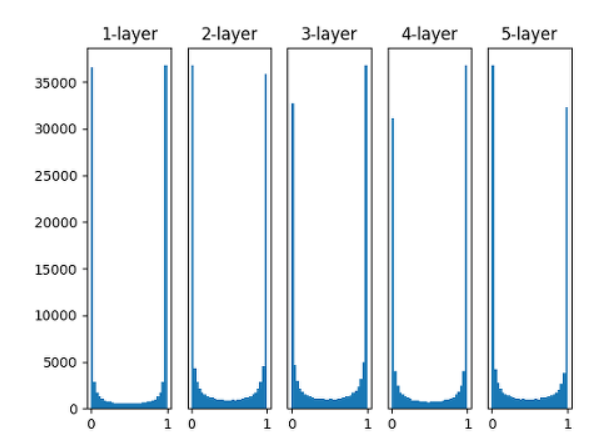
\includegraphics[page={1},width=0.45\textwidth]{./intro/sigmoid_normal1.PNG}}
				\quad
				\subfloat[N(0, 0.0001)]
				{\includegraphics[page={2},width=0.45\textwidth]{./intro/sigmoid_normal2.PNG}}
				\caption{Initial Values Following Normal Distribution}
				\label{fig:signormal}
			\end{figure}
		\end{itemize}
	\end{frame}	


	\begin{frame}{Importance of initialization}
		\begin{itemize}
			\item The result of Figure~\ref{fig:signormal} is the distribution of $Y = \sigma(XW + b).$ after each hidden layer.
			\item Each notation follows:
			\begin{enumerate}
				\vspace{3pt}
				\item $Y$ is an output.
				\item $\sigma(\cdot)$ is a sigmoid function.
				\item $X$ is an input.
				\item $W$ is a parameter matrix which is initialized.
				\item $b$ is a bias term which is initialized with 0.
				\vspace{3pt}
			\end{enumerate}	
			\item Since the intercept term is an added value, it can be initialized to 0.
			\item The (a) of Figure~\ref{fig:signormal} has eventually gradient vanishing because of being distributed many 0 and 1 values.
			\item The (b) of Figure~\ref{fig:signormal} does not happen gradient vanishing, but loses the advantage of using nodes a lot.
		\end{itemize}
	\end{frame}	


	\section{Various Initialization Mehotds}
	\begin{frame}{1. RBM \& DBM}
		\begin{itemize}
			\item Restricted Boltzmann Machine(RBM)\cite{rbm} is a generative stochastic artificial neural network proposed by Professor Hinton in 2006.
			\item It is mainly used to determine the initial value and works like unsupervised learning.
			\item As it is complicated, RBM is not used well these days.
			\vspace{10pt}
			\begin{figure}[h]
				\centering
				\subfloat[Forward]
				{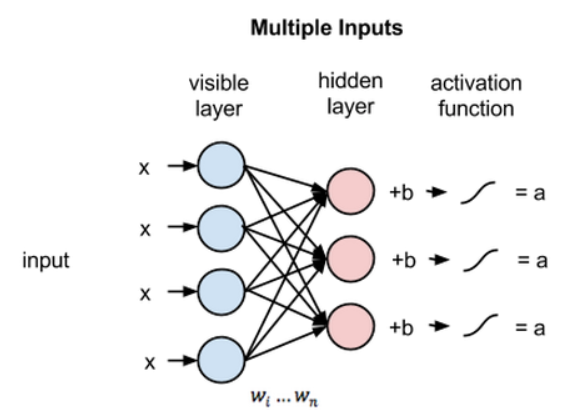
\includegraphics[page={1},width=0.4\textwidth]{./rbm,dbm/rbm0.PNG}}
				\quad
				\subfloat[Backward]
				{\includegraphics[page={2},width=0.45\textwidth]{./rbm,dbm/rbm1.PNG}}
				\caption{RBM}
				\label{fig:rbm}
			\end{figure}
		\end{itemize}
	\end{frame}


	\begin{frame}{1. RBM \& DBM}
		\begin{itemize}
			\item "Restricted" means no connection between nodes in each layer.
			\item Also, calculate $W$ by training until the difference between the input and the result of Figure~\ref{fig:rbm} (a) and (b) is small.
			\item RBM slightly is distinguished from the Autoencoder in using different bias term in Figure~\ref{fig:rbm} (a) from in Figure~\ref{fig:rbm} (b).
			\item And last, if you stack multiple RBM, you get Deep Boltzmann Machine(DBM).
			\item On a lighter note, Deep Belief Network(DBN) is made with the initial values of DBM.
		\end{itemize}
	\end{frame}	


	\begin{frame}{1. RBM \& DBM}
		\begin{itemize}
			\item The DBM can be seen in the figure below.
			\vspace{10pt}
			\begin{figure}[h]
				\centering
				\subfloat[Keep]
				{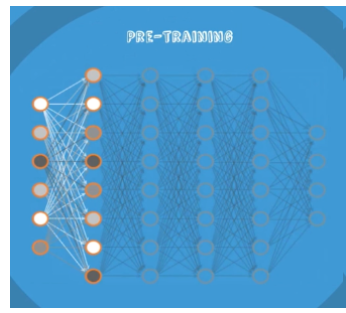
\includegraphics[page={1},width=0.28\textwidth]{./rbm,dbm/rbm2_pretraining_1.PNG}}
				\quad
				\subfloat[Going]
				{\includegraphics[page={2},width=0.28\textwidth]{./rbm,dbm/rbm2_pretraining_2.PNG}}
				\quad
				\subfloat[On]
				{\includegraphics[page={3},width=0.28\textwidth]{./rbm,dbm/rbm2_pretraining_3.PNG}}
				\caption{DBM}
				\label{fig:dbm}
			\end{figure}
		\end{itemize}
	\end{frame}


	\begin{frame}{1. RBM \& DBM}
		\begin{itemize}
			\item Finally, you can use the $W$, parameter matrix, obtained in this way as the initial value for the training model.
			\item This initial values assignment is also called 'Fine Tuning'.
			\vspace{10pt}
			\begin{figure}[h]
				\centering
				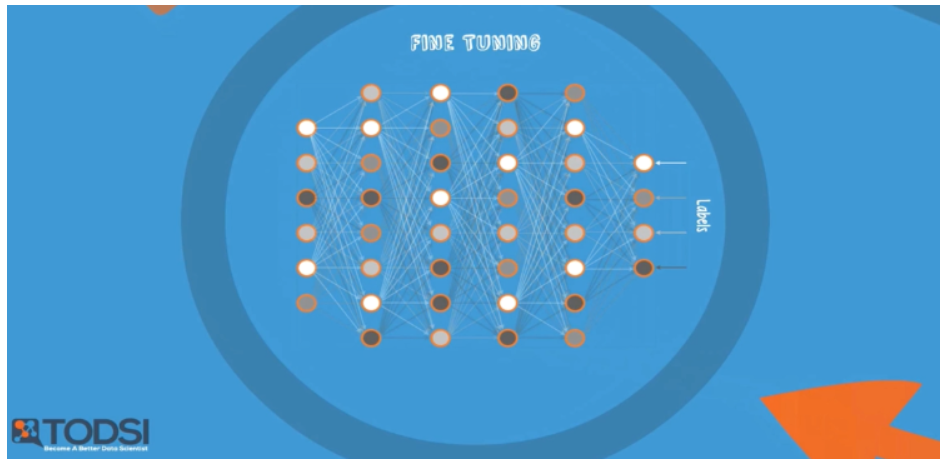
\includegraphics[scale=0.4]{./rbm,dbm/rbm3_finetuning.PNG}	
				\caption{Fine Tuning}
				\label{fig:dbm2}	
			\end{figure}
		\end{itemize}
	\end{frame}	


	\begin{frame}{2. Simple Uniform Initialization}
		\begin{itemize}
			\item Very simply, you can give the initial values to follow the uniform distribution.
			\vspace{10pt}
			\begin{gather*}
			W\text{'s elements} \sim U(-0.5,0.5)  
			\end{gather*}
			\item Absolutely, it is not used nowadays.
			\item Note that $W$ is a parameter matrix.
		\end{itemize}
	\end{frame}	


	\begin{frame}{3. LeCun Initialization}
		\begin{itemize}
			\item Also known as the founder of the LeNet and the father of CNN, Yann LeCun suggests giving the following initial values:
			\item LeCun method\cite{lecun} have not be used well recently since ReLU came out.
			\vspace{10pt}
			\begin{enumerate}
				\vspace{3pt}
				\item LeCun Normal Initialization
				\begin{gather*}
					W\text{'s elements} \sim N(0,\sigma^2) \quad , \quad \sigma = \sqrt{\frac{1}{n_{in}}}  
				\end{gather*}
				\vspace{3pt}
				\item LeCun Uniform Initialization
				\begin{gather*}
					W\text{'s elements} \sim U(-a,a) \quad , \quad a = \sqrt{\frac{3}{n_{in}}}  
				\end{gather*}
				\vspace{3pt}
			\end{enumerate}	
			\item Note that $n_{in}$ is the number of previous layer nodes.
		\end{itemize}
	\end{frame}	


	\begin{frame}{3. LeCun Initialization}
		Pf)
		\begin{itemize}
		\item Let $n$=number of input nodes , $x$=input, $Y$=output, $w$=weight. ($w,x,Y$ : R.V. \& independent each other) 
		\item And, let's not consider the activation function. Then,
		\begin{gather*}
			Y = w_1 x_1 + w_2 x_2 + \cdots + w_n x_n
		\end{gather*}
		\item Thus, variance of $Y$ is:
		\begin{align*}
			Var[Y] &= Var[\sum_{i=1}^{n}{w_i x_i}] \\ &= n\left[ E[x_i]^2Var[w_i]+E[w_i]^2 Var[x_i] + Var[w_i]Var[x_i] \right]
		\end{align*}
		\end{itemize}
	\end{frame}	


	\begin{frame}{3. LeCun Initialization}
		Pf)
		\begin{itemize}
			\item Let the mean of $x$ and $w$ be 0. Then,
			\begin{gather*}
				Var[Y] = n Var[w_i]Var[x_i] 
			\end{gather*}
			\item Therefore, in order to maintain the variance of $x$ and $Y$, the variance of $w_i$ must be $\frac{1}{n}$.
			\item In the end, the appropriate initialization values for normal and uniform distributions are set.
		\end{itemize}
	\end{frame}	


	\begin{frame}{4. Xavier(Glorot) Initialization}
		\begin{itemize}
			\item It is the initialization method that Xavier Glorot first proposed in 2010\cite{glorot}.
			\item It is still widely used as an initialization method unless otherwise specified.
			\vspace{10pt}
			\begin{enumerate}
				\vspace{3pt}
				\item Xavier Normal Initialization
				\begin{gather*}
				W\text{'s elements} \sim N(0,\sigma^2) \quad , \quad \sigma = \sqrt{\frac{1}{(n_{in}+n_{out})/2}}  
				\end{gather*}
				\vspace{3pt}
				\item Xavier Uniform Initialization
				\begin{gather*}
				W\text{'s elements} \sim U(-a,a) \quad , \quad a = \sqrt{\frac{3}{(n_{in}+n_{out})/2}}  
				\end{gather*}
				\vspace{3pt}
			\end{enumerate}	
			\item $n_{in}$  : the number of previous layer nodes.
			\item $n_{out}$ : the number of next layer nodes.
		\end{itemize}
	\end{frame}	


	\begin{frame}{4. Xavier(Glorot) Initialization}
		\begin{itemize}
			\item Xavier(or Glorot) initialization is effective when using tanh or sigmoid as an activation function.
			\vspace{10pt}
			\begin{figure}[h]
				\centering
				\subfloat[Distribution Trend]
				{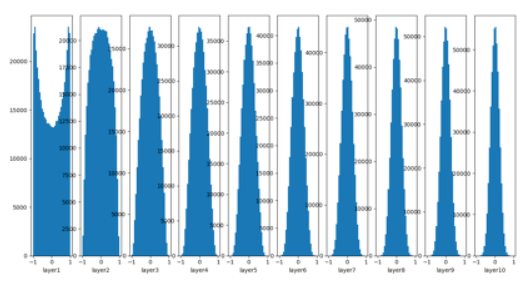
\includegraphics[page={1},width=0.45\textwidth]{./cnn/xavier/sigmoid_xavier2.PNG}}
				\quad
				\subfloat[Mean \& Std.]
				{\includegraphics[page={2},width=0.45\textwidth]{./cnn/xavier/sigmoid_xavier1.PNG}}
				\caption{Xavier with Sigmoid}
				\label{fig:sigxavier}
			\end{figure}
		\end{itemize}
	\end{frame}


	\begin{frame}{4. Xavier(Glorot) Initialization}
		\begin{itemize}
			\item However, it is not effective when using ReLU as an activation function.
			\vspace{10pt}
			\item So we use the He initialization, which will be explained in the next slide.
			\begin{figure}[h]
				\centering
				\subfloat[Distribution Trend]
				{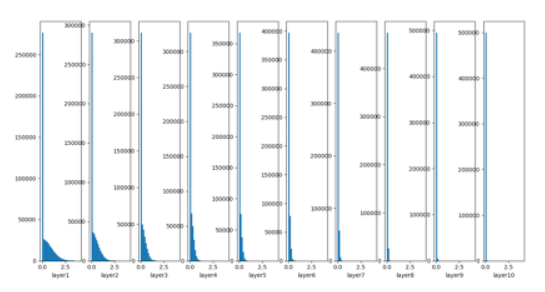
\includegraphics[page={1},width=0.45\textwidth]{./cnn/xavier/relu_xavier2.PNG}}
				\quad
				\subfloat[Mean \& Std.]
				{\includegraphics[page={2},width=0.45\textwidth]{./cnn/xavier/relu_xavier1.PNG}}
				\caption{Xavier with ReLU}
				\label{fig:reluxavier}
			\end{figure}
		\end{itemize}
	\end{frame}


	\begin{frame}{5. He Initialization}
		\begin{itemize}
			\item It is the initialization method that Kaiming He first proposed in 2015\cite{he}.
			\item He initialization is used a lot in the CNN models with ReLU.
			\vspace{10pt}
			\begin{enumerate}
				\vspace{3pt}
				\item He Normal Initialization
				\begin{gather*}
				W\text{'s elements} \sim N(0,\sigma^2) \quad , \quad \sigma = \sqrt{\frac{2}{n_{in}}}  
				\end{gather*}
				\vspace{3pt}
				\item He Uniform Initialization
				\begin{gather*}
				W\text{'s elements} \sim U(-a,a) \quad , \quad a = \sqrt{\frac{2\times 3}{n_{in}}}  
				\end{gather*}
				\vspace{3pt}
			\end{enumerate}	
			\item $n_{in}$  : the number of previous layer nodes.
			\item $n_{out}$ : the number of next layer nodes.
		\end{itemize}
	\end{frame}	


	\begin{frame}{5. He Initialization}
		\begin{itemize}
			\item The difference from Xavier initialization is that the output node is not taken into account and the variance of the initial value is doubled.
			\item The reason for doubling the variance comes from a simple statistical calculation that takes into account the form of $Y = max(0,x)$.
			\vspace{10pt}
			\begin{figure}[h]
				\centering
				\subfloat[Distribution Trend]
				{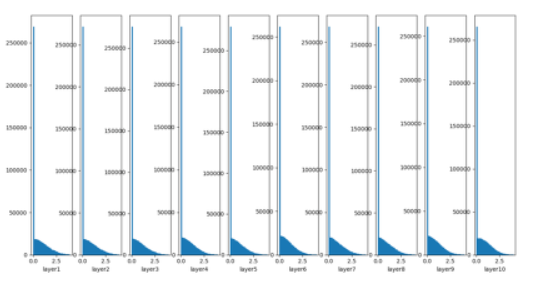
\includegraphics[page={1},width=0.45\textwidth]{./cnn/he/relu_he2.PNG}}
				\quad
				\subfloat[Mean \& Std.]
				{\includegraphics[page={2},width=0.45\textwidth]{./cnn/he/relu_he1.PNG}}
				\caption{He with ReLU}
				\label{fig:reluhe}
			\end{figure}
		\end{itemize}
	\end{frame}

	
	\begin{frame}{5. He Initialization}
		Showing)
		\begin{itemize}
			\item Let $x$=output before applying activation function, $Y$=final output. ($Y=max(0,x)$, i.e. $Y=x+$ReLU  ) 
			\item Also, $x,Y$ : R.V. \& independent each other. 
			\item And let's look at the relationship between $Y$'s variance and $x$'s variance. 
			\item Thus, variance of $Y$ is:
			\begin{align*}
			V[Y] &= V[X\cdot I(X>0)] \\ 
			&= V[X] + V[X\cdot I(X \le 0)] - 2Cov[X,X\cdot I(X \le 0)] \\
			&= V[X] - V[X\cdot I(X \le 0)]
			\end{align*}
		\end{itemize}
	\end{frame}	
	
	
	\begin{frame}{5. He Initialization}
		Showing)
		\begin{itemize}
			\item That is,
			\begin{gather*}
			V[X\cdot I(X>0)] = V[X] - V[X\cdot I(X \le 0)]
			\end{gather*}
			\item Assuming symmetry for $x=0$, 
			\begin{gather*}
			V[Y] = \frac{1}{2} V[X]
			\end{gather*}
			\item In combination with what we got in slide 13, we multiply the variance of the initial value by 2 to make the output distribution safe.
		\end{itemize}
	\end{frame}	


	\section{Interim Summary}
	\begin{frame}{Interim Summary}
		\begin{itemize}
			\item The summary is as follows :
			\vspace{10pt}
			\begin{figure}[h]
				\centering
				\subfloat[Sigmoid]
				{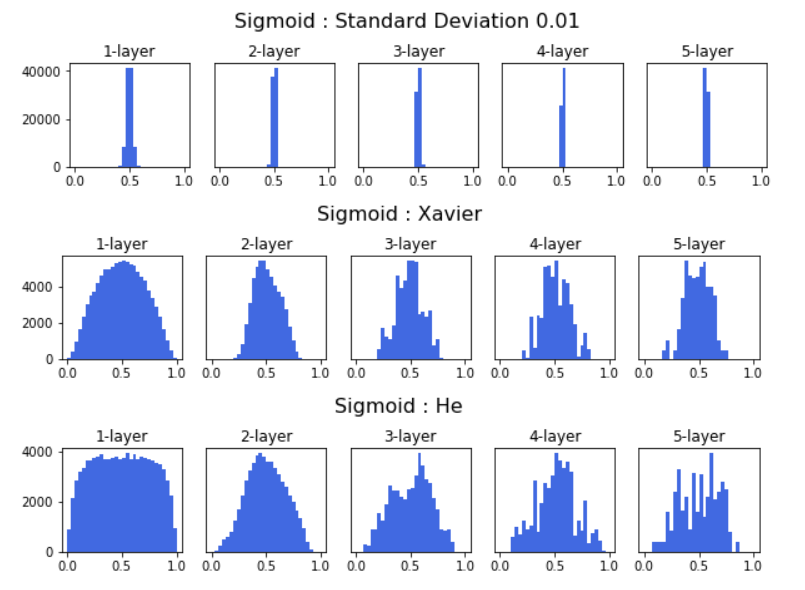
\includegraphics[page={1},width=0.45\textwidth]{./cnn/cnn_sigmoid.PNG}}
				\quad
				\subfloat[Tanh]
				{\includegraphics[page={2},width=0.45\textwidth]{./cnn/cnn_tanh.PNG}}
				\caption{Various Initialization Methods with Sigmoid \& Tanh}
				\label{fig:cnnsigmoidtanh}
			\end{figure}
		\end{itemize}
	\end{frame}


	\begin{frame}{Interim Summary}
		\begin{figure}[h]
			\centering
			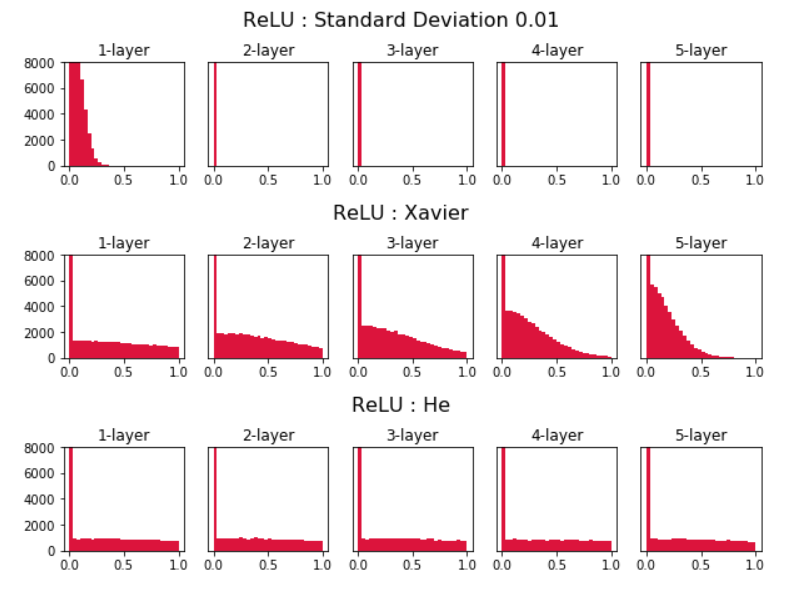
\includegraphics[scale=0.6]{./cnn/cnn_relu.PNG}	
			\caption{Various Initialization Methods with ReLU}
			\label{fig:cnnrelu}	
		\end{figure}
	\end{frame}


	\begin{frame}{Interim Summary}
		\begin{itemize}
			\item Finally, in the end, the initialization is performed in the following distribution.
			\vspace{10pt}
			\begin{figure}[h]
				\centering
				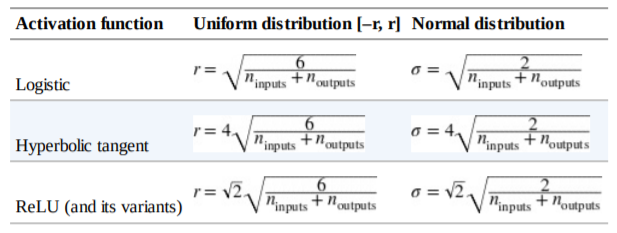
\includegraphics[scale=0.6]{./etc/init.PNG}	
				\caption{Various Initialization Methods}
				\label{fig:initialzing}	
			\end{figure}
			\item To learn more, see 'Aurélien Géron(2017), Hands-On Machine Learning with Scikit-Learn and TensorFlow'.
		\end{itemize}
	\end{frame}


	\section{Various initialization methods in RNN}
	\begin{frame}{6. Other Initialization Methods}
		\begin{itemize}
			\item The three initialization methods I will introduce are mainly used in RNN.
			\vspace{8pt}
			\begin{enumerate}
				\item Orthogonal\cite{orthogonal} : This is how you initialize using the Singular Value Decomposition(SVD). If $W=U\Lambda V^T$ then $W$ is randomly generated from the standard normal distribution, 
				and $U$ calculated through the SVD is used as the initial value. Especially, it works well on RNN.
				\vspace{8pt}
				\item Le et al.\cite{rnnrelu} : This is the initialization method used with ReLU. By giving $\boldsymbol{W=I}$ and $\boldsymbol{b=0}$ to their initial values, they start off ordinarily at first learning.
				\vspace{8pt}
				\item Talathi et al.\cite{rnnrelu2} : This is the initialization method used with ReLU. It is explained specifically in the next slide.
			\end{enumerate}
		\end{itemize}
	\end{frame}	


	\begin{frame}{6. Other Initialization Methods}
		\begin{itemize}
			\item Talathi et al., hypothesize that an initialization where one eigenvalue is equal to 1 and the rest are less than 1 is better. 
			\item Talathi et al. initialization is as follows:
			\vspace{7pt}
			\begin{enumerate}
				\item Sample a matrix $\bf{A}$ $\in R^{N \times N}$ whose values are drawn from $N(0,1)$ and $N$ is the number of units in the RNN.
				\vspace{5pt}
				\item Compute $\bf{B}$ $=\frac{1}{N}$ $\bf{A}{A^T}$ and let $\lambda_{max}$ be the the largest eigenvalue of the matrix $\bf{B+I}$.
				\vspace{5pt}
				\item Initialize $\bf{W}$ $= \frac{1}{\lambda_{max}}$ $\bf{B + I}$.
			\end{enumerate}
			\vspace{7pt}
			\item Empirically this is better than initializing $\bf{W=I}$.
		\end{itemize}
	\end{frame}	


	\section{Conclusion}
	\begin{frame}{Conclusion}
		\begin{itemize}
			\item Initialization methods are still being studied as a major concern.
			\item Batch Normalization(BN) has the effect of making the initialization method less important.
			\item For the initial value distribution, there is no clear usage criteria for normal and uniform distribution.
			\item Nevertheless, we use nomral initialization rather than uniform, and in the case of CNN, we almost always use a combination of 'He initialization + ReLU'.
		\end{itemize}
	\end{frame}


	\section{Next Time}
	\begin{frame}{Next}
		\begin{itemize}
			\item Next time, we'll deal with the followings:
			\vspace{7pt}
			\begin{enumerate}
				\item Type of loss function.
				\item More complex CNN models.
				\item About the GAN.
			\end{enumerate}
			\vspace{7pt}
			\item Of course, Python code learning proceeds at the same time.
		\end{itemize}
	\end{frame}
	
	
	\section{Reference}
	\begin{frame}[allowframebreaks]{Reference}
		\bibliography{references}
	\end{frame}


\end{document}
